\section{Recurso solar}\label{sec:recurso}

\subsection{Diagrama cilíndrico}

La posición del Sol se calculó con la declinación $\delta$, el ángulo horario $\omega=15^\circ(t_s-12)$, donde $t_s$ es el tiempo solar, y la latitud $\phi=\SI{9.936}{\degree}$:
\begin{equation}
\sin h = \sin\phi\,\sin\delta + \cos\phi\,\cos\delta\,\cos\omega,
\end{equation}
\begin{equation}
\sin\alpha = \frac{\cos\delta\,\sin\omega}{\cos h},
\end{equation}
donde $h$ es la altura solar y $\alpha$ el acimut medido desde el sur (en la figura se expresa desde el norte, en sentido horario). La Fig.~\ref{fig:cilindrico} presenta el diagrama cilíndrico del sitio para el día 21 de cada mes.

\begin{figure*}[!t]
\centering
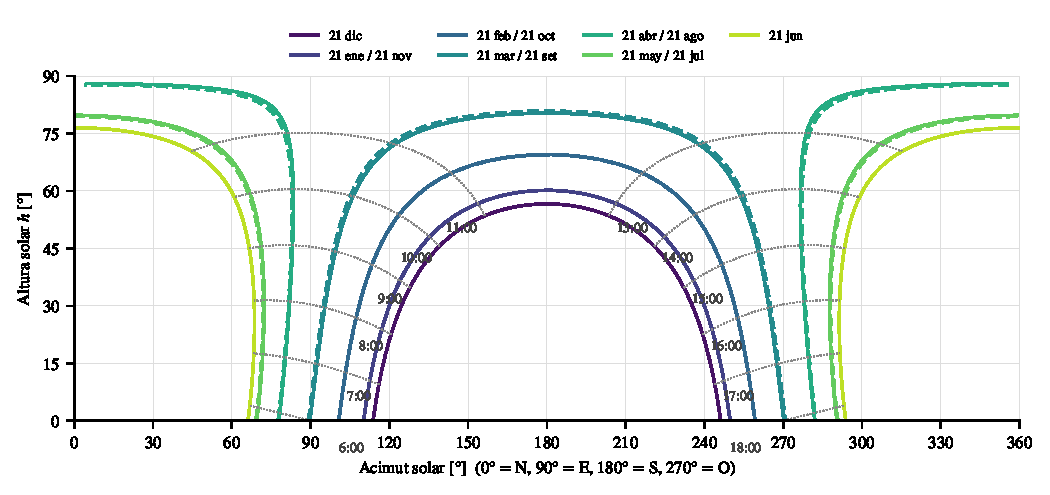
\includegraphics[width=0.95\textwidth]{diagrama_cilindrico.pdf}
\caption{Diagrama cilíndrico del recorrido solar en Santa Rosa de Oreamuno (\SI{9.936}{\degree}\,N), día 21 de cada mes, en tiempo solar. Las líneas punteadas unen puntos de la misma hora.}
\label{fig:cilindrico}
\end{figure*}

Por la cercanía al ecuador, el Sol pasa alto todo el año: al mediodía solar la altura es de \SI{56.6}{\degree} el 21 de diciembre, la menor del año, y de \SI{80.3}{\degree} el 21 de marzo. Entre abril y agosto el Sol pasa al norte del cenit y en el resto del año, al sur. El día dura entre \SI{11.4}{h} y \SI{12.6}{h}. Como el Sol sale por el este todo el año, la cara este del techo recibe sol directo desde el amanecer, y la cara oeste desde el mediodía.

\subsection{Radiación solar}

La radiación se obtuvo de PVGIS 5.3, con la base PVGIS-ERA5 de 2005 a 2023 y el horizonte calculado con el modelo de elevación del terreno \cite{pvgis}. Se consultó la irradiación sobre el plano horizontal, sobre las dos caras del techo (\SI{12}{\degree} al este y \SI{12}{\degree} al oeste), sobre un plano de \SI{12}{\degree} al sur y sobre el plano óptimo que calcula PVGIS. La Tabla~\ref{tab:radiacion} presenta los promedios diarios de cada mes, expresados en horas solares pico (HSP), y la Fig.~\ref{fig:radiacion} los grafica.

\begin{table}[!htb]
\caption{Irradiación diaria media por mes [HSP = kWh/(m$^2\cdot$día)] y temperatura media}
\label{tab:radiacion}
\centering
\footnotesize
\setlength{\tabcolsep}{3.5pt}
\begin{tabular}{l c c c c c c}
\toprule
Mes & Horizontal & \SI{12}{\degree} este & \SI{12}{\degree} oeste & \SI{12}{\degree} sur & Óptimo & $T_{\mathrm{media}}$ [\si{\celsius}] \\
\midrule
Ene & 5.02 & 5.03 & 4.88 & 5.59 & 5.56 & 16.3 \\
Feb & 5.69 & 5.73 & 5.50 & 6.11 & 6.12 & 16.5 \\
Mar & 5.88 & 5.94 & 5.65 & 6.01 & 6.07 & 17.1 \\
Abr & 5.47 & 5.54 & 5.23 & 5.34 & 5.43 & 18.1 \\
May & 4.44 & 4.55 & 4.22 & 4.22 & 4.35 & 18.6 \\
Jun & 4.24 & 4.36 & 4.02 & 3.99 & 4.11 & 18.6 \\
Jul & 4.28 & 4.35 & 4.08 & 4.05 & 4.15 & 18.2 \\
Ago & 4.41 & 4.51 & 4.18 & 4.26 & 4.37 & 18.3 \\
Set & 4.38 & 4.49 & 4.14 & 4.38 & 4.48 & 18.4 \\
Oct & 3.85 & 3.94 & 3.66 & 4.00 & 4.06 & 18.2 \\
Nov & 3.68 & \textbf{3.73} & 3.54 & 3.97 & 3.98 & 17.5 \\
Dic & 4.45 & 4.46 & 4.33 & 5.00 & 4.95 & 16.8 \\
\midrule
Año [kWh/m$^2$] & 1695 & 1721 & 1623 & 1728 & 1750 & \\
\bottomrule
\end{tabular}
\\[2pt]
{\footnotesize Fuente: PVGIS 5.3, PVGIS-ERA5 2005--2023 \cite{pvgis}. Óptimo: \SI{14}{\degree} de inclinación y acimut de \SI{-40}{\degree} (hacia el sureste).}
\end{table}

\begin{figure}[!htb]
\centering
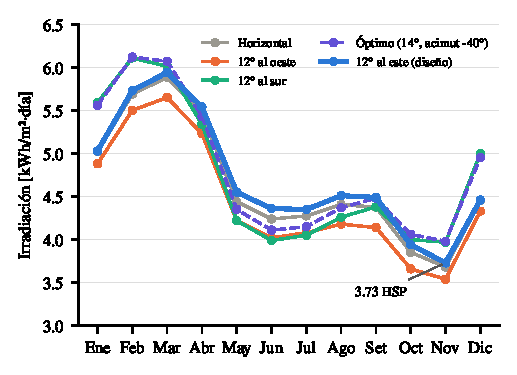
\includegraphics[width=\anchofig]{radiacion_mensual.pdf}
\caption{Irradiación diaria media por mes en distintos planos (PVGIS).}
\label{fig:radiacion}
\end{figure}

Se distinguen dos épocas: sobre la cara este, de diciembre a abril la irradiación diaria está entre 4.46 y \SI{5.94}{HSP}, y de mayo a noviembre baja a valores de 3.73 a \SI{4.55}{HSP}, con el mínimo en noviembre. En ese periodo la fracción difusa media de PVGIS sube de 0.26--0.34 a 0.43--0.49, lo que corresponde a la época lluviosa \cite{pvgis}.

\subsection{Ángulo óptimo y plano de diseño}

PVGIS calcula como óptimo un plano de \SI{14}{\degree} de inclinación con acimut de \SI{-40}{\degree}, que recibe \SI{1750}{kWh/m^2} al año \cite{pvgis}. La cara este del techo, con \SI{12}{\degree}, recibe \SI{1721}{kWh/m^2}, solo 1.7\,\% menos, y la cara oeste \SI{1623}{kWh/m^2}, 5.6\,\% menos que la cara este. Por eso los módulos se colocan en la cara este, paralelos al techo: una estructura que los orientara al óptimo ganaría 1.7\,\% de energía a cambio de más material y más carga de viento sobre la lámina.

En un sistema aislado el dimensionamiento se hace con el mes de menor radiación, porque el banco debe recargarse también en ese mes. Sobre la cara este ese mes es noviembre, con \SI{3.73}{HSP}. En noviembre el plano óptimo recibiría \SI{3.98}{HSP}, 6.7\,\% más, pero la diferencia no cambia la cantidad de módulos (Sección~\ref{sec:aislado}).
